\documentclass[]{article}
\usepackage[margin=1in, portrait]{geometry}
%\usepackage{fullpage}
\usepackage{amsmath}
\usepackage{amssymb}
\usepackage{amsthm}
\usepackage{mathrsfs}
\usepackage[english]{babel}
\usepackage{multirow}
\usepackage{graphicx}
\newtheorem{stel}{Stelling}
\usepackage{float}
\usepackage{textcomp}
\usepackage{footmisc}
\usepackage[colorlinks=true, urlcolor=blue, linkcolor=blue, citecolor=blue, pdfborder={0 0 0}, linktoc=page]{hyperref}
\setlength{\parindent}{0 pt}
\usepackage{etoolbox}
\usepackage{scrextend}

\newcommand{\ba}{\begin{addmargin}[9mm]{0cm}}
\newcommand{\ea}{\end{addmargin}}
\newcommand{\cm}{\color{blue} \hspace{3mm}}



\title{\vspace{0cm} \huge \textsc{3D-RT: 3D Radiative Transfer} \\
                \vskip3mm \textsc{Code Documentation} }

\author{\large Frederik De Ceuster}

\date{}

\begin{document}

\maketitle

\vskip5cm

\begin{abstract}
This report gives an overview of some technical aspects of the 3D-RT code. The goal is to motivate why and explain how some things are coded the way they are.
\end{abstract}

\vskip5cm

\tableofcontents

\newpage


\section{General}

3D-RT is a multipurpose accelerated 3D radiative transfer code. Given a gas with a density and velocity distribution, an external radiation field and a provisional chemical composition, it selfconsistently calculates the temperature, level populations and chemical composition of the gas. 3D-RT is a ray-tracing code, meaning that to solve for the transport of electromagnetic radiation, the radiative transfer equation is solved along a set of rays.

\bigskip

The first version of 3D-RT is mainly based on 3D-PDR \cite{3DPDR}. The main difference is that in 3D-RT the radiative transfer is solved exactly and not in the Sobolev or large velocity gradient (LVG) approximation.

\bigskip

The code is mainly written in C with some features of C++. For the ray tracing the discretization scheme of the unit sphere is used from HEALPix\footnote{\url{https://healpix.jpl.nasa.gov}}. The chemical rate equations are solved using the CVODE solver provided in SUNDIALS\footnote{\url{https://computation.llnl.gov/projects/sundials}}. Most of the linear algebra is done using the Eigen\footnote{\url{http://eigen.tuxfamily.org}} library.



\section{Some general structures}

\subsection{Storing multi-dimensional arrays as lists}

All multi-dimensional arrays in the code are stored as one-dimensional lists. On the lowest level, this is the case in every computer code. However, we chose to explicitly write the one-dimensional lists and define the relations between list index and the rows and columns.

\section{Ray tracing}

To be able to simulate 3-dimensional objects we need a way to represent them in computer language. In this first verison of the code space is dicretized into a truely unstructered grid. In a truely unstructered grid every point is stored separately, without any relation between different points. Physical quantities as the position, gas velocity and temperature are stored independent for every point. In a later version we aim to exploit more the possible structure of the grid.

\bigskip

Space is discretized into \texttt{ngrid} grid points.

\subsection{Efficiently storing the evaluation points}

THE ORIGIN IS NOT AN EVALUATION POINT!

\texttt{raytot[RINDEX(n,r)]} gives the total number of evaluation points on a ray \texttt{r} through a gridpoint \texttt{n}. Here the origin is not counted as an evaluation point. Otherwise we would store the origin each time as an evaluation point, resulting in \texttt{ngrid} times \texttt{NRAYS} unnecessary doubles. In the radiative transfer part of the code we do want to consider the origin as an eveluation point. Therefore we will systematically add one to \texttt{raytot} in that part of the code.

\subsection{Equivalent rays}
of

\section{Radiative transfer}

\begin{figure}[H]
	\centering
	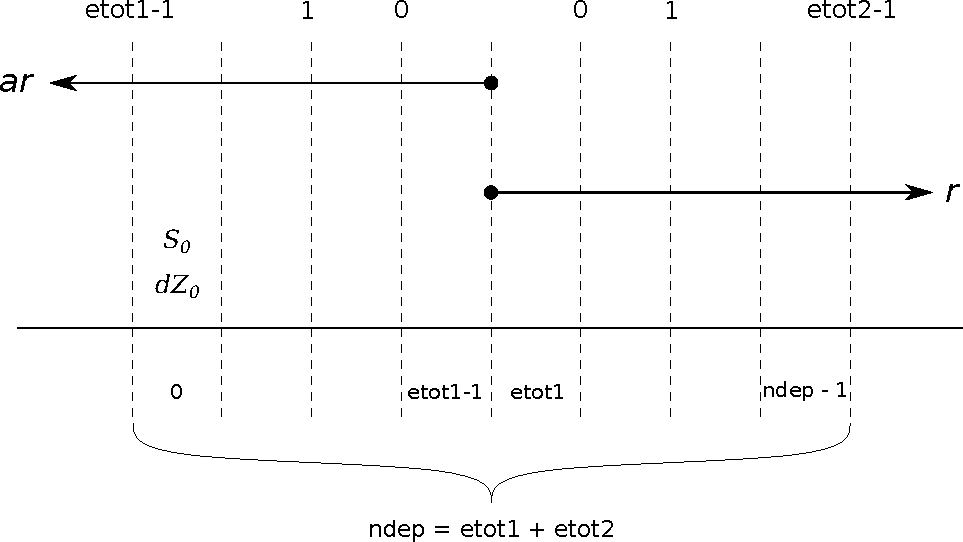
\includegraphics[scale=.8]{Images/ray.pdf}
	\caption{Construction of the ray along wich the radiative transfer is solved.}
	\label{grid}
\end{figure}


\subsection{\texttt{exact\_feautrier} solver}

Based on the benchmarks, we can conclude that the \texttt{exact\_feautrier} solver has a 9 digit precission.


\newpage

\bibliography{library}
\bibliographystyle{ieeetr}



\end{document}
